\section{Model-to-text transformation}
\label{sec:m2t}

In the following section, we present the \hilecop{} model-to-text
transformation (HM2T) through its formal specification. The goal of
the transformation is to generate a \hvhdl{} design that implements an
input SITPN model. To obtain an output design with the same behavior
than the input model, the execution semantics of SITPNs must be
encoded in terms of \vhdl{} code. To achieve this, the place and the
transition designs have been defined. The behavior of these two
designs, given in Appendices~\ref{app:place-design} and
\ref{app:trans-design}, correspond to a place-centered and
transition-centered implementation of the SITPN semantics in
\vhdl{}. At the moment of the transformation, instances of the place
and the transition designs, referred to as PDIs and TDIs, will be
created for each place and transition of the input model. Then, these
subcomponents of the output design's behavior will be interconnected
through their port interface.  While the SITPN execution semantics is
scattered in the internal behavior of PDIs and TDIs, the
interconnection of these instances permits us to obtain the global
behavior of the input model at runtime (or at least, that is what we
want to prove). Moreover, the interpretation elements of the input
SITPN model, namely the conditions, actions and functions will be
implemented by the input and output ports of the output design. The
conditions will be translated into Boolean input ports (referred to as
condition ports) in the generated design. The transition-condition
associations will be implemented by the interconnections between
condition ports and the interface of transition design instances
(TDIs). The activation/execution status of actions/functions will be
reflected by the value of the Boolean output ports (referred to as
action and function ports) of the generated design. The transformation
will generate two processes, namely the \texttt{actions} and
\texttt{functions} processes, that will be responsible for the
assignment of values to the action and function ports.

There exists a mapping between the elements of the input SITPN model
and their corresponding version in the generated \hvhdl{} design. This
mapping is captured within a structure called a SITPN-to-\hvhdl{}
binder.  This structure is generated alongside the transformation of
the input SITPN model into a \hvhdl{} design. It is both useful to
express the HM2T and its formal
specification. Definition~\ref{def:sitpn-to-hvhdl-binder} formally
describes the SITPN-to-\hvhdl{} binder structure:
\begin{definition}[SITPN-to-\hvhdl{} design binder]
  \label{def:sitpn-to-hvhdl-binder}
  Given a $sitpn\in{}SITPN$ and a \hvhdl{} design $d\in{}design$, a
  SITPN-to-\hvhdl{} binder $\gamma\in{}WM(sitpn,d)$ is a record
  ${<}PMap,TMap,CMap,AFMap{>}$ where:
  \begin{itemize}
  \item $PMap\in{}P\rightarrow{}\{id_p~|~\mathtt{comp}(id_p,\mathtt{place},g,i,o)\in{}d.beh\}$
  \item $TMap\in{}T\rightarrow{}\{id_t~|~\mathtt{comp}(id_t,\mathtt{transition},g,i,o)\in{}d.beh\}$
  \item $CMap\in\mathcal{C}\rightarrow\{id_c~|~(\mathtt{in}, id_c, \mathtt{bool})\in{}d.ports\}$
  \item $AFMap\in\mathcal{A}\cup\mathcal{F}\rightarrow\{id_{af}~|~(\mathtt{out}, id_{af}, \mathtt{bool})\in{}d.ports\}$
  \end{itemize}
\end{definition}

For a given binder $\gamma$ and an element of an SITPN structure
$e\in{}P\cup{}T\cup\mathcal{C}\cup\mathcal{A}\cup\mathcal{F}$, we
write $\gamma(e)$ where $e$ is looked up in the appropriate
function. For instance, for a given $f\in\mathcal{F}$, $\gamma(f)$ is
a shorthand notation for $AFMap(f)$ where $\gamma={<}\dots,AFMap{>}$.

\bigskip

The formal specification of the HM2T is expressed as a relation
between the inputs of the transformation, namely a SITPN model and a
bounding function, and its outputs, which can be either a pair
composed of a \hvhdl{} design and a SITPN-to-\hvhdl{} binder or the
error value. The relation is written
$HM2T_{\mathtt{spec}}\subseteq{}SITPN\times(P\rightarrow\mathbb{N})\times{}((design\times{}WM(sitpn,d))\cup\{\mathtt{err}\})$
where $sitpn$ and $d$ refer to the first and the third parameters of
the relation. As hinted at the beginning of the section, specifying
the HM2T is mostly about describing how the PDIs and TDIs are
interconnected through their port interface. The error case arises
when the input SITPN model does not respect the well-definition
property (cf. Definition~\ref{def:wd-sitpn}).

The bounding function, that is, the second parameter of the
$HM2T_{\mathtt{spec}}$ relation, associates each place of the SITPN
model with a bound in terms of number of tokens.  A bound represents
the maximum number of tokens that a place will possibly hold at some
point of the execution of the model. We assume that these bounds have
been computed through the formal analysis of the input SITPN model. Of
course, the existence of such a function implies that all the SITPN
models that are passed as inputs to the HM2T are \textit{bounded}
models\footnote{There exists no place that can accumulate an unlimited
  number of tokens in the course of the execution of the model.}. As a
matter of fact, we can prove that the HM2T is not semantic-preserving
when the input is an unbounded SITPN model. The execution of such a
model will lead to an infinite incrementation of the number of tokens
in a given place. This infinite incrementation, while valid in the
mathematical world, can never be mirrored by a \vhdl{} implementation
of the model where all values must be finite. Therefore, the behavior
of the SITPN model and its \hvhdl{} implementation will diverge at a
certain point of their execution.

\bigskip

Definition~\ref{def:hm2t-spec} presents the formal specification of
the HM2T through a selected set of points. The full definition of the
HM2T's formal specification can be found in
\cite{Iampietro2022hfspec}. Each point of the definition will be
commented and illustrated as and when they arise. We have implemented
the $HM2T_{\mathtt{spec}}$ relation in \coq{}, and have written a
\coq{} function, named \texttt{sitpn2hvhdl}, that implements the
transformation but is yet to be proved sound and complete regarding
its specification. In Definition~\ref{def:hm2t-spec}, we also refer to
the names of generic constants and signals declared in the place and
transition designs. To achieve conciseness, we use aliases to refer to
these constants and signals. The correspondence between the aliases
and the full names is given in Appendix~\ref{sec:cnsts-sigs-names}.

%%%%% Definition for the HM2T formal specification. %%%%%

\def\pdiInBeh{\mathtt{comp}(\gamma(p),\mathtt{place},g_p,i_p,o_p)\in{}d.beh}
\def\tdiInBeh{\mathtt{comp}(\gamma(t),\mathtt{transition},g_t,i_t,o_t)\in{}d.beh}
\def\tdiInBehP#1{\mathtt{comp}(\gamma(#1),\mathtt{transition},g_{#1},i_{#1},o_{#1})\in{}d.beh}

\begin{definition}[\hilecop{} model-to-text transformation specification]
  \label{def:hm2t-spec}
  For all SITPN model $sitpn\in{}SITPN$, bounding function
  $b\in{}P\rightarrow\mathbb{N}$, \hvhdl{} design $d\in{}design$, and
  SITPN-to-\hvhdl{} binder $\gamma\in{}WM(sitpn,d)$, we have
  $HM2T_{\mathtt{spec}}(sitpn,b,(d,\gamma))$ if:
  \begin{enumerate}
  \item\label{it:pdi-tdi-only} All design instantiation statement in
    the design's behavior
    either creates a PDI or a TDI: \\
    $\forall{}id_c,id_e,g,i,o~s.t.~\mathtt{comp}(id_c,id_e,g,i,o)\in{}d.beh,~id_e=\mathtt{place}\lor{}id_e=\mathtt{transition}$.
    
  \item\label{it:actions-functions-only} The \texttt{actions} and
    \texttt{functions} processes are the
    only two processes in the design's behavior:\\
    $\forall{}id_p,vars,ss~s.t.~\mathtt{ps}(id_p,vars,ss)\in{}d.beh,~id_p=\mathtt{actions}\lor{}id_p=\mathtt{functions}$.
    
  \item\label{it:d-is-elaborable} Design $d$ is elaborable in the context of the \hilecop{} design store\footnote{The \hilecop{} design store is a specific design store that holds the definition of the \texttt{place} and \texttt{transition} designs.} and given an empty dimensioning function:\\
    $\exists{}\Delta\in{}ElDesign,\sigma_e\in\Sigma$ s.t.
    $\mathcal{D_\mathcal{H}},\emptyset\vdash{}d\xrightarrow{elab}\Delta,\sigma_e$.
    
  \item\label{it:binder-bij} All the fields of the SITPN-to-\hvhdl{} binder are bijective
    functions: $PMap(\gamma)$ is bijective, $TMap(\gamma)$ is
    bijective,\dots
  \end{enumerate}

  \bigskip
  
  Points~\ref{it:pdi-tdi-only} to \ref{it:binder-bij} specify the
  global shape of the output design $d$ and the binder structure
  $\gamma$.  Point~\ref{it:pdi-tdi-only} states that the behavior of
  design d is only composed of place or transition design
  instances. Point~\ref{it:actions-functions-only} states that there
  are only two processes in the behavior of the output design, namely
  the $\mathtt{actions}$ process and the $\mathtt{functions}$
  process. The content of the \texttt{actions} process is specified in
  Point~\ref{it:actions}. Point~\ref{it:d-is-elaborable} states that
  the output design is elaborable, i.e. syntactically well-formed,
  statically well-typed, with no multiply-driven signals, etc.
  Point~\ref{it:binder-bij} states that there is a one-to-one
  correspondence between the elements of the input SITPN model and the
  elements of the output design and that this correspondence is
  established through the binder $\gamma$.

  \bigskip
  
  \begin{enumerate}[resume]
  \item\label{it:pdi-exists} For all place of the input SITPN model,
    there exists a corresponding PDI identified through $\gamma$ in
    the behavior of the output
    design:\\
    $\forall{}p\in{}P,\exists{}g_p,i_p,o_p$ s.t.  $\pdiInBeh$.
    
  \item\label{it:pdi-gmap} For all place of the input SITPN model and
    its corresponding PDI, the generic map of the PDI holds the
    following associations:
    \begin{equation*}
      \begin{aligned}
        \forall{}p\in&{}P,g_p,i_p,o_p, \\
        & \pdiInBeh\Rightarrow \\
        &
          \begin{aligned}
            g_p=\{&(\mathtt{mm}\Rightarrow{}b(p)), \\
                  & (\mathtt{ian}\Rightarrow
                    \begin{cases}
                      1~\mathrm{if}~\mathtt{input}(p)=\emptyset \\
                      \vert{}\mathtt{input}(p)\vert~\mathrm{otherwise} \\
                    \end{cases}), \\
                  &(\mathtt{oan}\Rightarrow
                    \begin{cases}
                      1~\mathrm{if}~\mathtt{output}(p)=\emptyset \\
                      \vert{}\mathtt{output}(p)\vert~\mathrm{otherwise} \\
                    \end{cases})\} \\
          \end{aligned} \\
      \end{aligned}
    \end{equation*}
    where
    \texttt{input}$(p)=\{t~\vert~post(t,p)=\lfloor\omega\rfloor\}$,
    the set of input transitions of place $p$, and
    \texttt{output}$(p)=\{t~\vert~pre(p,t)=\lfloor(\omega,a)\rfloor\}$,
    the set of output transitions of place $p$.
    
  \item\label{it:pdi-im} For all place of the input SITPN model and
    its corresponding PDI, there is an association between the
    \texttt{im} input port and the initial marking of the place in the
    input port map of the PDI:\\
    $\forall{}p\in{}P,g_p,i_p,o_p,\pdiInBeh{}$
    $\Rightarrow(\mathtt{im}\Rightarrow{}M_0(p))\in{}i_p$.
  \end{enumerate}

  \bigskip

  Point~\ref{it:pdi-exists} states the existence of a corresponding
  PDI in the behavior of the output design for each place of the input
  SITPN model. Point~\ref{it:pdi-gmap} describes how the content of
  the generic map of a PDI is computed based on the properties of the
  corresponding place. Note that the \texttt{mm} constant,
  corresponding to the maximal marking of the PDI, receives its value
  from the bounding function. Point~\ref{it:pdi-im} describes how the
  initial marking of the place is reflected on the input port map of
  the corresponding PDI through the \texttt{im} input
  port. Figure~\ref{fig:gen-pci-ex} illustrates the link between the
  number of input and output arcs of a place and how this information
  is passed through the generic map and impacts the dimensioning of
  the corresponding PDI's port interface.

  \begin{figure}[h]
    \centering
    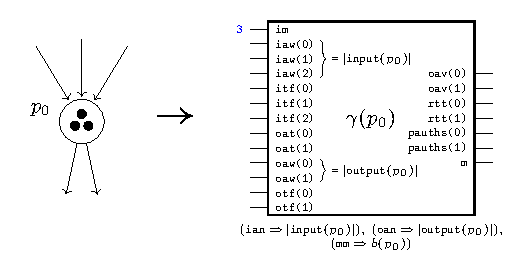
\includegraphics[keepaspectratio,width=.7\textwidth]{gen-pci-ex.eps}
    \caption{A graphical representation of the interface of the PDI
      $\gamma(p_0)$ (on the right) implementing place $p_0$ (on the
      left). The generic map associations appear underneath the PDI.}
    \label{fig:gen-pci-ex}
  \end{figure}
  
  \begin{enumerate}[resume]

  \item\label{it:exists-tdi} For all transition of the input SITPN model, there exists a
    corresponding TDI identified through $\gamma$ in the behavior of
    the output design:\\
    $\forall{}t\in{}T,\exists{}g_t,i_t,o_t$ s.t. $\tdiInBeh$.
    
  \item\label{it:tdi-gen-map} For all transition of the input SITPN model and its
    corresponding TDI, the generic map of the TDI holds the following
    associations:
    \begin{equation*}
      \begin{aligned}[t]
        \forall{}t&\in{}T,g_t,i_t,o_t, \\
                  & \tdiInBeh\Rightarrow \\
                  &
                    \begin{aligned}[t]
                      g_t=\{&(\mathtt{tt}\Rightarrow{}
                      \begin{cases}
                        \mathtt{not\_temp}~\mathrm{if}~t\notin{}\mathtt{dom}(I_s) \\
                        \mathtt{temp\_a\_a}~\mathrm{if}~I_s(t)=[a,a] \\
                        \mathtt{temp\_a\_b}~\mathrm{if}~I_s(t)=[a,b] \\
                        \mathtt{temp\_a\_inf}~\mathrm{if}~I_s(t)=[a,\infty] \\
                      \end{cases}),\\
                      & (\mathtt{mtc}\Rightarrow
                      \begin{cases}
                        1~\mathrm{if}~t\notin{}\mathtt{dom}(I_s) \\
                        b~\mathrm{if}~I_s(t)=[a,b] \\
                        a~\mathrm{if}~I_s(t)=[a,\infty] \\
                      \end{cases}), \\
                      & (\mathtt{ian}\Rightarrow
                        \begin{cases}
                          1~\mathrm{if}~\mathtt{input}(t)=\emptyset \\
                          \vert{}\mathtt{input}(t)\vert~\mathrm{otherwise} \\
                        \end{cases}), 
                      (\mathtt{cn}\Rightarrow
                      \begin{cases}
                        1~\mathrm{if}~\mathtt{conds}(t)=\emptyset \\
                        \vert{}\mathtt{conds}(t)\vert~\mathrm{otherwise} \\
                      \end{cases})\}. \\
                    \end{aligned} \\
      \end{aligned}
    \end{equation*}
    where
    \texttt{input}$(t)=\{p~\vert~pre(p,t)=\lfloor(\omega,a)\rfloor\}$,
    the set of input places of transition $t$, and
    \texttt{conds}$(t)=\{c~\vert~\mathbb{C}(t,c)=1\lor\mathbb{C}(t,c)=-1\}$,
    the set of conditions associated with transition $t$.
    
  \item\label{it:tdi-time-itval} For all transition of the input SITPN
    model and its corresponding TDI, the input port map of the TDI
    holds the following associations:
    \begin{equation*}
      \begin{aligned}[t]
        \forall{}t&\in{}T,g_t,i_t,o_t, \\
                  & \tdiInBeh\Rightarrow \\
                  &
                    \begin{aligned}[t]
                      \{&(\mathtt{A}\Rightarrow\begin{cases}
                                                0~\mathrm{if}~t\notin\mathtt{dom}(I_s) \\
                                                l(I_s(t))~\mathrm{otherwise} \\
                                              \end{cases}), \\
                      & (\mathtt{B}\Rightarrow\begin{cases}
                                              0~\mathrm{if}~t\notin\mathtt{dom}(I_s)\lor{}u(I_s(t))=\infty \\
                                              u(I_s(t))~\mathrm{otherwise} \\
                                            \end{cases})\}\subseteq{}i_t. \\
                    \end{aligned}
        \\
      \end{aligned}
    \end{equation*}

  \end{enumerate}

  \bigskip

  Similarly to the case of places, Points~\ref{it:exists-tdi} to
  \ref{it:tdi-time-itval} state the existence of a corresponding TDI
  for each transition of the input model, and specify how its generic
  map and its input port map must be built regarding the properties of
  the transition, namely: the shape of the time interval, the number
  of input arcs, the number of associated
  conditions. Figure~\ref{fig:gen-tdi-ex} illustrates how the
  properties of a transition are implemented in the interface of the
  corresponding TDI.

  \begin{figure}[h]
    \centering
    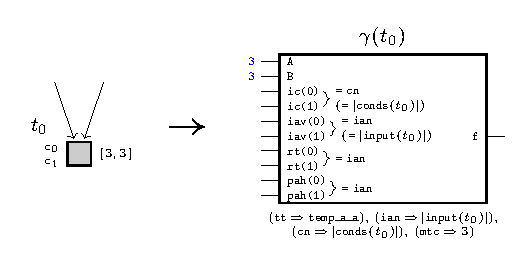
\includegraphics[keepaspectratio,width=.8\textwidth]{gen-tdi-ex.eps}
    \caption{A graphical representation of the interface of the TDI
      $\gamma(t_0)$ (on the right) implementing transition $t_0$ (on
      the left). The generic map associations appear underneath the
      TDI.}
    \label{fig:gen-tdi-ex}
  \end{figure}
  
  \begin{enumerate}[resume]        
  \item\label{it:post-arc} For all post arc of the input SITPN model,
    the TDI and PDI corresponding to the source transition and target
    place of the arc are connected as follows:
    \begin{equation*}
      \begin{aligned}[t]
        \forall{}t&\in{}T,p\in{}P,g_t,i_t,o_t,g_p,i_p,o_p,\omega\in\mathbb{N}^{*}, \\
                  & post(t,p)=\lfloor\omega\rfloor\Rightarrow \\
                  & \tdiInBeh\Rightarrow \\
                  & \pdiInBeh\Rightarrow\\
                  &
                    \begin{aligned}[t]
                      \exists{}i & \in[0,\vert\mathtt{input}(p)\vert-1]~s.t.~(\mathtt{iaw}(i)\Rightarrow\omega)\in{}i_p \\
                                 & \land\exists{}id_s~s.t.~(id_s,\mathtt{bool})\in{}d.sigs
                                   \land(\mathtt{fired}\Rightarrow{}id_s)\in{}o_t\land(\mathtt{itf}(i)\Rightarrow{}id_s)\in{}i_p. \\
                    \end{aligned}
        \\
      \end{aligned}
    \end{equation*}
  \end{enumerate}
  
  \bigskip

  In Point~\ref{it:post-arc}, $(id_s,\mathtt{bool})\in{}d.sigs$
  indicates the signal $id_s$ is declared as a Boolean internal signal
  in the output design. Figure~\ref{fig:gen-post-arc} illustrates the
  translation of a post arc of the input SITPN model as described in
  Point~\ref{it:post-arc}. The weight of the arc is passed to the PDI
  through the \texttt{iaw} (for \texttt{input\_arcs\_weights}) input
  port. In the behavior of the output design, all arc information is
  encoded through the input port interface of PDIs. All computations
  that necessitate the arc information, such as the marking update or
  the setting of time counter reset signals, are performed in the
  behavior of the place design. Therefore, only the PDIs need to hold
  the arc information.

  \begin{figure}[h]
    \centering
    \includegraphics[keepaspectratio,width=.7\textwidth]{gen-post-arc.eps}
    \caption{The translation of a post arc, connecting a transition
      $t_0$ to a place $p_0$, into an interconnection between the
      interfaces of the corresponding TDI and PDI.}
    \label{fig:gen-post-arc}
  \end{figure}
  
  \begin{enumerate}[resume]
  \item\label{it:pre-arc} For all pre arc of the input SITPN model,
    the PDI and TDI corresponding to the source place and target
    transition of the arc are connected as follows:
    \begin{equation*}
      \begin{aligned}[t]
        \forall{}t&\in{}T,p\in{}P,g_t,i_t,o_t,g_p,i_p,o_p,\omega\in\mathbb{N}^{*},a\in\{\mathtt{basic},\mathtt{test},\mathtt{inhib}\}, \\
                  & pre(p,t)=\lfloor(\omega,a)\rfloor\Rightarrow \\
                  & \tdiInBeh\Rightarrow \\
                  & \pdiInBeh\Rightarrow\\
                  & \exists{}i\in[0,\vert\mathtt{output}(p)\vert-1]~s.t.~\{(\mathtt{oaw}(i)\Rightarrow\omega),(\mathtt{oat}(i)\Rightarrow{}a)\}\subseteq{}i_p \\
                  & \begin{aligned}[t]
                      \land\exists{}j &\in[0,\vert\mathtt{input}(t)\vert-1],id_{av},id_{rt},id_{frd},id_{pah}~s.t. \\
                                      & \{(id_{av},\mathtt{bool}),(id_{rt},\mathtt{bool}),(id_{frd},\mathtt{bool}),(id_{pah},\mathtt{bool})\}\subseteq{}d.sigs \\
                                      & \land(\mathtt{oav}(i)\Rightarrow{}id_{av})\in{}o_p\land(\mathtt{iav}(j)\Rightarrow{}id_{av})\in{}i_t \\
                                      & \land(\mathtt{rtt}(i)\Rightarrow{}id_{rt})\in{}o_p\land(\mathtt{rt}(j)\Rightarrow{}id_{rt})\in{}i_t \\
                                      & \land(\mathtt{otf}(i)\Rightarrow{}id_{frd})\in{}i_p\land(\mathtt{fired}\Rightarrow{}id_{frd})\in{}o_t \\
                                      & \land(\mathtt{pah}(i)\Rightarrow{}id_{frd})\in{}o_p \\
                                      & \land(a=\mathtt{test}\lor{}a=\mathtt{inhib}\lor{}\mathtt{confl}(p)=\emptyset\Rightarrow(\mathtt{pah}(j)\Rightarrow\mathtt{true})\in{}i_t) \\
                                      & \land(a=\mathtt{basic}\land{}\mathtt{confl}(p)\neq\emptyset~or~\mathtt{err}\Rightarrow(\mathtt{pah}(j)\Rightarrow{}id_{pah})\in{}i_t). \\
                    \end{aligned} \\
      \end{aligned}
    \end{equation*}
    where $\mathtt{confl}\in{}P\rightarrow{}2^T\cup\{\mathtt{err}\}$
    takes a place $p$ as input and yields either an error or an
    ordered set of transitions computed as follows:
    \begin{enumerate}
    \item If all conflicts between the output transitions of $p$ are
      solved by mutual exclusion, or if the set of conflicting
      transitions of $p$ is a singleton, then $\mathtt{confl}$ returns
      an empty set.
    \item Otherwise, the function tries to establish a total ordering
      over the set of conflicting transitions of $p$ w.r.t the firing
      priority relation:
      \begin{itemize}
      \item If no such ordering can be established (in that case, the
        firing priority relation is ill-formed, and the input SITPN is
        not well-defined), $\mathtt{confl}$ returns the \texttt{err}
        value.
      \item Otherwise, the function returns the set in a decreasing
        priority order.
      \end{itemize}
    \end{enumerate}
    
  \end{enumerate}

  \bigskip
  
  Figure~\ref{fig:gen-pre-arc} illustrates the translation of a pre
  arc of the input SITPN model as described in Point~\ref{it:pre-arc}.
  As for the post arcs, the arc information is passed through the
  input port map of the PDI. As there are three possible types of pre
  arc, the \texttt{oat} (for \texttt{output\_arcs\_types}) input port
  receives the arc type information.  In Figure~\ref{fig:gen-pre-arc},
  we assume that there remain some conflicts not solved by mutual
  exclusion in the set of output transitions of place
  $p_0$. Otherwise, according to Point~\ref{it:pre-arc}, the
  interconnection between $\mathtt{pah(i)}$ and $\mathtt{pah(j)}$
  would not be effective.
  
  \begin{figure}[h]
    \centering
    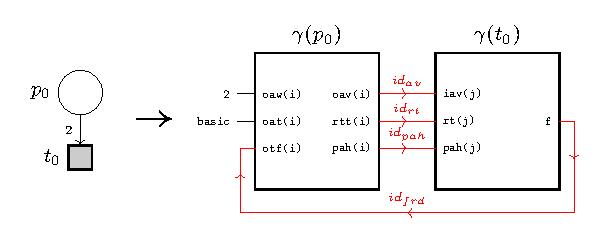
\includegraphics[keepaspectratio,width=.8\textwidth]{gen-pre-arc.eps}
    \caption{The translation of a pre arc, connecting a place $p_0$ to
      a transition $t_0$, into signal interconnections between the
      interfaces of the corresponding PDI and TDI. }
    \label{fig:gen-pre-arc}
  \end{figure}

  \begin{enumerate}[resume]
  \item\label{it:port-indices-ordering} For all place of the input
    SITPN model for which conflicts in its output transitions are not
    solved by mutual exclusion, the port indices of the corresponding
    PDI reflect the priority order established between the conflicting
    output transitions:
    \begin{equation*}
      \begin{aligned}[t]
        \forall{}p&\in{}P,t,t'\in{}\mathtt{confl}(p),g_p,i_p,o_p,g_t,i_t,o_t,g_{t'},i_{t'},o_{t'}, \\
                  & t\succ{}t'\Rightarrow\\
                  & \pdiInBeh\Rightarrow \\
                  & \tdiInBehP{t}\Rightarrow \\
                  & \tdiInBehP{t'}\Rightarrow \\
                  &
                    \begin{aligned}[t]
                      (\forall{}i,j&\in\mathbb{N},id_{frd},id_{frd'},id_{s},id_{s'},name_t,name_{t'},id_{out}, \\
                                   & (\mathtt{fired}\Rightarrow{}id_{frd})\in{}o_t\Rightarrow \\
                                   & (\mathtt{fired}\Rightarrow{}id_{frd'})\in{}o_{t'}\Rightarrow \\
                                   & \{(\mathtt{otf}(i)\Rightarrow{}id_{frd}),(\mathtt{otf}(j)\Rightarrow{}id_{frd'})\}\subseteq{}i_p\Rightarrow \\
                                   & (name_t\Rightarrow{}id_{s})\in{}i_t\Rightarrow \\
                                   & (name_{t'}\Rightarrow{}id_{s'})\in{}i_{t'}\Rightarrow \\
                                   & \{(id_{out}(i)\Rightarrow{}id_s),(id_{out}(j)\Rightarrow{}id_{s'})\}\subseteq{}o_p\Rightarrow \\
                                   & i<j) \\
                    \end{aligned} \\
      \end{aligned}
    \end{equation*}
  \end{enumerate}

  \bigskip

  As specified in Point~\ref{it:port-indices-ordering}, the port
  indices in the interface of a PDI must reflect the priority order
  established between its \textit{conflicting} TDIs. Of course, this
  is only mandatory for the ports connecting the PDI to its
  conflicting TDIs. Otherwise, the index order does not matter, for
  instance while reifying a post arc connection.
  Figure~\ref{fig:gen-prio-order} illustrates the ordering of the port
  indices in the interface of a PDI as described in
  Point~\ref{it:port-indices-ordering}.

  \begin{figure}[h]
    \centering
    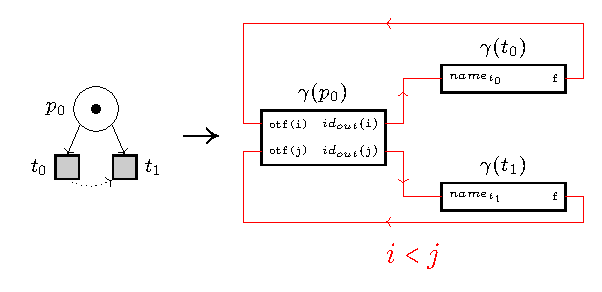
\includegraphics[keepaspectratio,width=.8\textwidth]{gen-prio-order.eps}
    \caption{Translation of the priority relation in terms of port
      index ordering. On the right, $name_{t_0}$ (resp. $name_{t_1}$)
      refers to any input port of TDI $\gamma(t_0)$
      (resp. $\gamma(t_1)$), and $id_{out}$ refers to any composite
      output port of PDI $\gamma(p_0)$. On the left, the dotted arc
      going from transition $t_0$ to $t_1$ indicates the $t_0$ has a
      higher firing priority than $t_1$. }
    \label{fig:gen-prio-order}
  \end{figure}

  \begin{enumerate}[resume]
  \item\label{it:actions} There exists an \texttt{actions} process
    that assigns a value to the output ports (referred to as
    \textit{action} ports) representing the activation status of the
    actions of the input SITPN model:
    
    $\exists{}ss_{ra},ss_{a}~s.t.~\mathtt{ps}(\mathtt{actions},\emptyset,\mathtt{rst}\{ss_{ra}\}\mathtt{else}\{\mathtt{falling}\{ss_a\}\})\in{}d.beh$
    and
    \begin{enumerate}
    \item The length of the $ss_{ra}$ and $ss_{a}$ sequences is equal
      to the number of actions of the input SITPN model:\\
      $\vert{}ss_{ra}\vert_{;}=\vert{}ss_a\vert_{;}=\vert\mathcal{A}\vert$
      where $\vert{}ss\vert{}_{;}=
      \begin{cases}
        \vert{}ss_1\vert_{;}+\vert{}ss_2\vert_{;}~\mathrm{if}~ss=ss_1;ss_2 \\
        1~\mathrm{otherwise}
      \end{cases}
      $
      
    \item During the initialization, all action ports are assigned to
      \texttt{false} by the \texttt{actions} process:
      $\forall{}a\in\mathcal{A},~\gamma(a)\Leftarrow\mathtt{false}\in{}ss_{ra}$
      
    \item An action port corresponding to an unassociated action is
      assigned to \texttt{false} during the falling edge
      phase:\\
      $\forall{}a\in\mathcal{A}~s.t.~\mathtt{pls}(a)=\emptyset,\gamma(a)\Leftarrow\mathtt{false}\in{}ss_{a}$
      where
      \texttt{pls}$(a)=\{p~\vert~\mathbb{A}(p,a)=\mathtt{true}\}$, the
      set of places associated with action $a$.
      
    \item Otherwise, the value of the action port is the result of the
      Boolean sum between the \texttt{marked} output port of all PDIs
      representing the places associated with the corresponding
      action:
      \begin{equation*}
        \begin{aligned}[t]
          \forall{}a&\in\mathcal{A},~\mathtt{pls}(a)\neq\emptyset\Rightarrow \\
                    &  \begin{aligned}[t]
                         \exists{}e_{or}& ~s.t.~\gamma(a)\Leftarrow{}e_{or}\in{}ss_a\land\mathtt{is\_bsum}(e_{or},\vert{}\mathtt{pls}(a)\vert) \\
                                        &
                                          \begin{aligned}
                                            \land\forall{}p& \in\mathtt{pls}(a),g_p,i_p,o_p, \\
                                                           & \pdiInBeh\Rightarrow \\
                                                           &
                                                             \begin{aligned}
                                                               \exists{}id_m& ~s.t.~(id_m,\mathtt{bool})\in{}d.sigs \\
                                                                            &\land{}id_m\in{}e_{or} \\
                                                                            & \land(\mathtt{marked}\Rightarrow{}id_m)\in{}o_p \\
                                                             \end{aligned} \\
                                          \end{aligned} \\
                       \end{aligned} \\
        \end{aligned}
      \end{equation*}
      where $\mathtt{is\_bsum}$ is defined as follows:

      \vspace{10pt}
      
      \begin{tabular}{l}
        {\begin{prooftree}
            \hypo{e\in{}\{id,b\}}
            \infer1{\mathtt{is\_bsum}(e,1)}
          \end{prooftree}} \\
      \end{tabular}
      \begin{tabular}{l}
        {\begin{prooftree}
            \hypo{\mathtt{is\_bsum}(e_1,n)}
            \hypo{\mathtt{is\_bsum}(e_2,m)}
            \infer2
            {\mathtt{is\_bsum}(\mathtt{or}(e_1,e_2),n+m)}
          \end{prooftree}} \\
      \end{tabular}
    \end{enumerate}
  \end{enumerate}

  \bigskip

  In Point~\ref{it:actions}, the $\mathtt{is\_bsum}$ relation states
  that a given expression is a Boolean sum (i.e. a composition of
  \texttt{or} expressions) of Boolean terminals or identifiers and
  that this expression has a given size. Through the \texttt{is\_bsum}
  relation, we want specify that all the internal signals connected to
  the \texttt{marked} ports of the associated PDIs are represented in
  the $e_{or}$ expression.  Figure~\ref{fig:gen-actions} describes the
  content of the \texttt{actions} process, obtained through the
  transformation of a given input SITPN model, as specified in
  Point~\ref{it:actions}. The specification of the \texttt{functions}
  process is very close to the definition of the \texttt{actions}
  process. The reader can find it in \cite{Iampietro2022hfspec}.
  
  \begin{figure}[!ht]
    \centering
    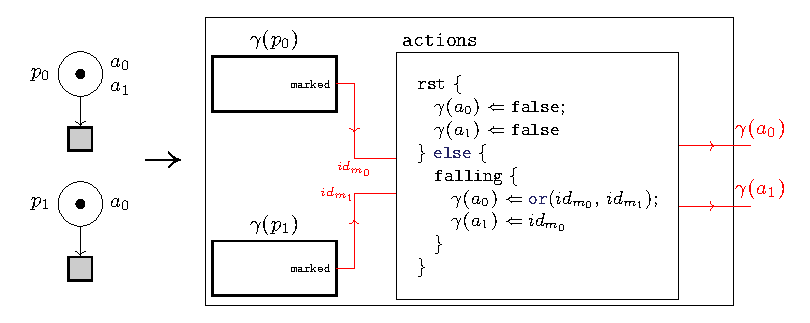
\includegraphics[keepaspectratio,width=\textwidth]{gen-actions.eps}
    \caption{The content of the \texttt{actions} process (on the
      right) based on the place-action associations of the input SITPN
      model (on the left). }
    \label{fig:gen-actions}
  \end{figure}

  \bigskip
  
  \begin{enumerate}[resume]
  \item\label{it:cond-ports} For all association between a transition and a condition, the
    input port (referred to as a \textit{condition} port) reflecting
    the Boolean value of the given condition is connected as follows
    to the input port map of the TDI corresponding to the associated
    transition:
    \begin{equation*}
      \begin{aligned}[t]
        \forall{}t&\in{}T,g_t,i_t,o_t,c\in\mathcal{C}, \\
                  & \tdiInBeh\Rightarrow \\
                  & (\mathbb{C}(t,c)=1\Rightarrow\exists{}i\in[0,\vert\mathtt{conds}(t)\vert-1]~s.t.~(\mathtt{ic}(i)\Rightarrow{}\gamma(c))\in{}i_t) \\
                  & (\mathbb{C}(t,c)=-1\Rightarrow\exists{}i\in[0,\vert\mathtt{conds}(t)\vert-1]~s.t.~(\mathtt{ic}(i)\Rightarrow{}\mathtt{not}(\gamma(c)))\in{}i_t). \\
      \end{aligned}
    \end{equation*}

  \end{enumerate}

  Figure~\ref{fig:gen-conds} illustrates the connection between a
  condition port and its associated TDIs as specified in
  Point~\ref{it:cond-ports}. Condition ports are connected to the
  \texttt{ic} (for \texttt{input\_conditions}) input port of their
  associated TDIs.
  
  \begin{figure}[h]
    \centering
    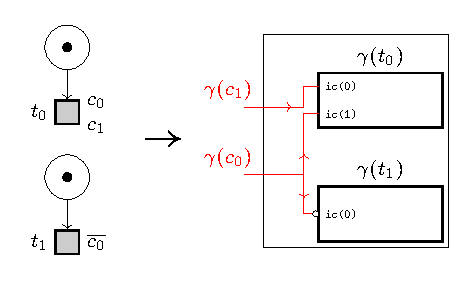
\includegraphics[keepaspectratio,width=.65\textwidth]{gen-conds.eps}
    \caption{Translation of the condition-transition associations (on
      the left) into interconnections between condition ports and
      TDIs' interfaces (on the right). }
    \label{fig:gen-conds}
  \end{figure}

  To conclude the definition of the $HM2T_{\mathtt{spec}}$ relation,
  we have $HM2T_{\mathtt{spec}}(sitpn,b,\mathtt{err})$ if $sitpn$ is
  not a well-defined SITPN model w.r.t. Definition~\ref{def:wd-sitpn}.
\end{definition}

%%% Local Variables:
%%% mode: latex
%%% TeX-master: "main"
%%% End:
